\section{GoTcha}
\label{sec:debug_arch}

\begin{figure*}
\centering
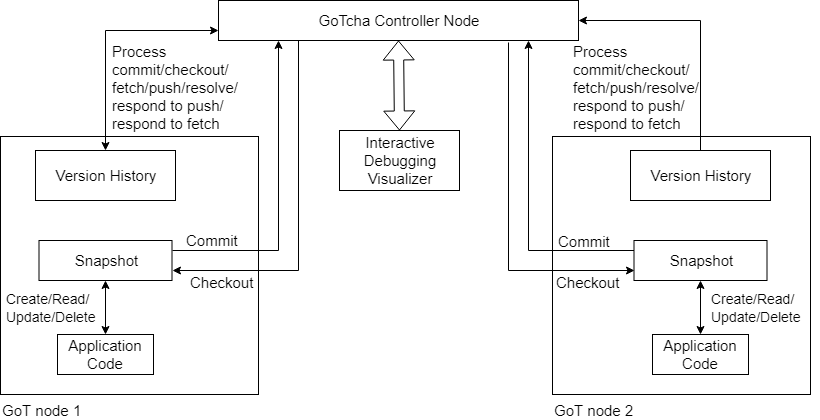
\includegraphics[width=0.85\textwidth]{images/debug_arch.png}
\caption{Architecture of GoTcha.}
\label{fig:proto_arch}
\end{figure*}

GoT nodes execute their tasks over shared objects that are stored in the version history in the dataframe. These version histories are primarily used, in GoT, to facilitate the communication between nodes using delta encoding and to detect and resolve conflicts. The version history is an internal component of the dataframe and is, therefore, typically not exposed to the programmer. 

In version control systems, the version histories are more than just a datastores for files. They document the evolution of the files stored in the repository over time. There are many tools available, such as GitKraken~\footnote{https://www.gitkraken.com} and SourceTree~\footnote{https://www.sourcetreeapp.com/}, that expose this evolution to users. Observing the version history, through these tools, not only tells us the current state of the repository, but also all the changes that were made to the repository in the past and in the order that they were made. This same principle can be leveraged in GoT, to expose the version history of object changes to the user. A debugger for GoT can expose the version history allowing users to observe the evolution of the state at a node, and detect errors that have already occurred. In addition to viewing errors in the version history, live and interactive debugging becomes possible, as the updates to the version history is driven explicitly by the application code, and performed via a small API in the dataframe (see Table~\ref{tbl:api}). By taking control of these APIs and giving this control of the execution to the user, the user can stop the application, observe the state of the version history at each node, resume and observe the change of state over the execution of the dataframe operations. This, along with the ability to observe variations in the order of execution, will assist the user in observing errors as they occur. 

We created an interactive debugger called GoTcha, to expose the changes made to the version history at each node in a Spacetime application. In this section, we explain the features of GoTcha. We will continue to use the distributed word frequency counter example, detailed in the previous section, to showcase the features of the debugger.

% Whats the debug environment.
For the purpose of the example, a test input file was created consisting of six lines, each with one word -- see Listing~\ref{lst:test_file}. The word frequencies for the words foo, bar, and baz are one, four, and one respectively. The application consists of two WordCounter nodes and one Grouper node that are launched in different machines. During execution, as shown in Listing~\ref{lst:grouper}, the Grouper node adds six Line objects and two Stop objects into its dataframe, and waits for the Stop objects to be accepted by the WordCounter nodes (Listing~\ref{lst:grouper}). WordCounter1 reads, tokenizes, and counts words on lines 1, 3, and 5. WordCounter2 does the same for lines 2, 4, and 6. Finally, both WordCounter nodes accept their Stop objects, and execution completes. The expected output is shown in Listing~\ref{lst:expected}. However, a different output is observed, shown in Listing~\ref{lst:observed}. The observed output is wrong, and this is where GoTcha can help.

\begin{figure*}%[htb]
% \centering
  \begin{subfigure}[b]{0.3\linewidth}
        \begin{lstlisting}[language=Python,basicstyle=\small,
        label=lst:test_file, captionpos=b, caption=Input file.]
        foo
        bar
        bar
        baz
        bar
        bar
        \end{lstlisting}
  \end{subfigure}
  \begin{subfigure}[b]{.3\linewidth}
        \begin{lstlisting}[language=Python,basicstyle=\small,
        label=lst:expected, captionpos=b, caption=Expected output.]
        foo 1
        bar 4
        baz 1
        \end{lstlisting}
  \end{subfigure}
  \begin{subfigure}[b]{.3\linewidth}
        \begin{lstlisting}[language=Python,basicstyle=\small,
        label=lst:observed, captionpos=b, caption=Observed output.]
        foo 1
        bar 6
        baz 1
        \end{lstlisting}
  \end{subfigure}
\end{figure*}


\subsection{Operation}
% how is GoTcha setup.
GoTcha follows the centralized service approach, discussed in Section~\ref{sec:design}, to have complete control over the nodes and expose the version history to the user at each node. This central service is an application by itself and is launched before any application nodes are launched. We call this application the GoTcha Controller Node (GCN from now on). The GCN is a web service to both the User Interface (UI), and the nodes in the application. When GoT nodes are launched in debug mode, they register themselves with the GCN. 

% What happens in debug mode.
When in debug mode, the architecture of the application is modified from what is shown in Figure~\ref{fig:gotnode} to what is shown in Figure~\ref{fig:proto_arch}. The primitives that read or write from the version history at each GoT node ({\em commit}, {\em checkout}, {\em fetch}, {\em push}) are all rerouted through the GCN. With each interaction, the version history at each node is also sent to the GCN to be shown to the users. While a traditional interactive debugger for a single threaded application would observe the change of state between each line of code, GoTcha observes state changes over each action of read or write performed on the version history at each node.

% Where does it start
At the start of the debugging session, after every node has been launched in debug mode, the user is shown the network topology of the application, as shown in Figure~\ref{fig:start_screen}. In this figure, on the left, the user sees that two WordCounter nodes (WordCounter1 and WordCounter2) and one Grouper node are being controlled by the GCN. The Grouper node is the authoritative node in the application, with both the WordCounter nodes making {\em fetch} and {\em push}  requests to the Grouper node. On the right, there is an input field for the user to add one or many breakpoint conditions to the debugger. The breakpoint condition shown here, returns True if there exists any WordCount object with the count dimension set to six, in the dataframe, at any GoT node.

\begin{figure*}
\centering
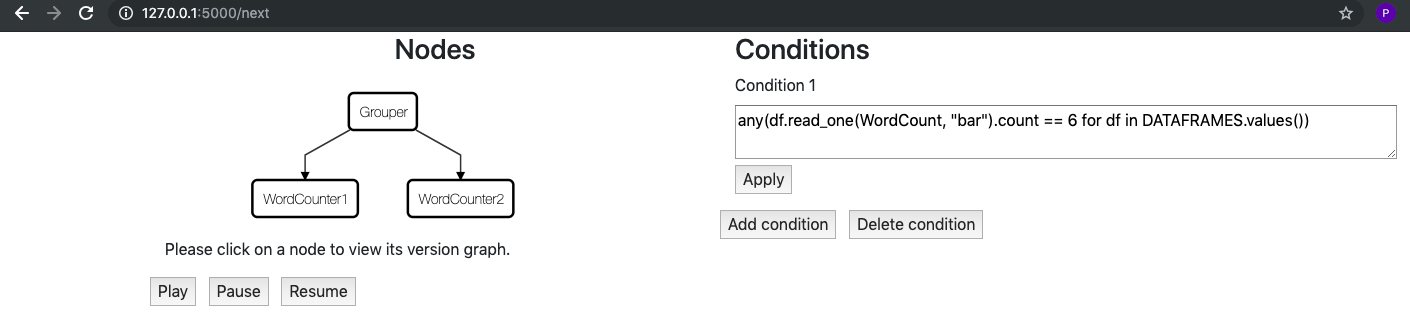
\includegraphics[width=\textwidth]{images/start_screen.png}
\caption{Debugger showing the network topology of the application.}
\label{fig:start_screen}
\end{figure*}

\subsection{Observing Node State}

\begin{figure*}
\centering
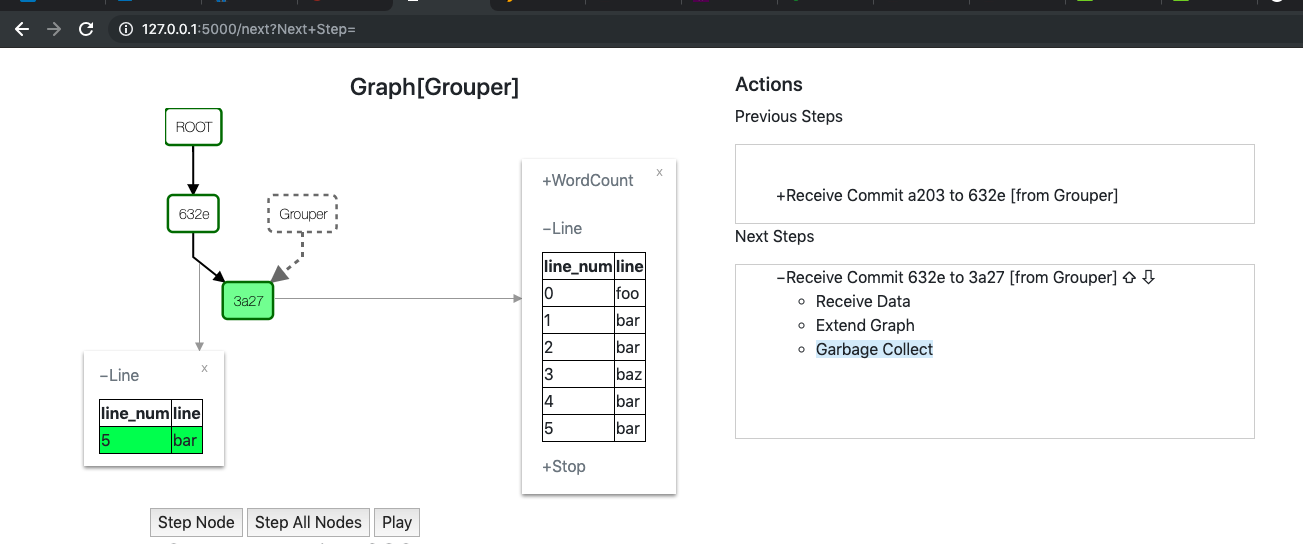
\includegraphics[width=\textwidth]{images/grouper_after_commit.png}
\caption{Debugger view showing version history at the end of a {\em commit}.}
\label{fig:after_commit}
\end{figure*}

% What is the node view.
The current version history of any node can be observed by clicking on the node in the topology graph in Figure~\ref{fig:start_screen}. Figure~\ref{fig:after_commit} shows the node view of the Grouper node, observing the result of the execution of the {\em commit} primitive at line 5 of Listing~\ref{lst:grouper} (during the last iteration of that loop). The version history is shown on the top left. The history shows three versions: ROOT, 632e, and 3a27. 3a27 happened-after 632e which in turn happened-after ROOT (the start version of every version history). The HEAD version of the graph, highlighted in green, is 3a27. 

% How to see the state.
Selecting the version brings up a tooltip that shows in tabular form, the state of objects at that version. The tooltip shows that the state at version 3a27 has six objects of type Line, and shows the values of the two dimensions (line\_num, line) for the Line objects. Though the tables for Stop and WordCounter have been collapsed, as shown by the plus shaped user interface element, there are no objects of those types present yet.

% How to see the change
Selecting the edge brings up a tooltip that shows the delta change (diff) associated with that edge. The diff associated with the edge 632e $\rightarrow$ 3a27 is also shown on the bottom left. In this case, the diff consists of a single object of type Line with the dimensions line\_num, and line having the values 5, and `bar' respectively. The entry is also marked in green, which signifies that the entry is a newly added object (added in line 4, Listing~\ref{lst:grouper}). Uncolored entries are considered to be modifications, and entries marked in red are considered to be deleted objects. The state of every version, and the diff associated with every edge can be observed. The dotted line relation shows us that the state of the snapshot of the Grouper node is known to be at version 3a27. 
% The version graph at each node includes the information of the last known state of each node that has communicated with it. In Grouper, since external nodes have not communicated yet, the only reference in the version graph is its own.

% How do we know what is being executed
On the right of Figure~\ref{fig:after_commit}, we see the state of the actions being executed on the dataframe at the Grouper node. The user sees both a list of previous steps that have been executed on the version history, and a list of steps that have to be executed (next steps). At the top of the next steps list is the current active step being executed. Each step directly maps to one of the dataframe primitives rerouted through GoTcha and is broken up into several phases. 

% More details on the current step.
We can see that the {\em commit} primitive has three phases. The first phase is receive data where a {\em commit} request is made using the diff staged in the snapshot. Stepping through this phase brings us to the extend graph phase, where the version history graph is extended from the HEAD version (632e) to the newly created version (3a27) and the new version is marked as the new HEAD. The last phase of commit, which is yet to be executed, is the garbage collect phase where obsolete versions in the graph (in this case 632e) are cleaned up.

% the dataframe primitive currently being executed. We see that the execution state is a Commit from version 632e to 3a27. It has already received data, extended the graph and is currently waiting to execute the garbage collection phase.

% How do we progress
At the bottom, we see three buttons: Step Node, Step All Nodes, and Play. Clicking on Step Node, would allow the garbage collect phase of {\em commit} at the Grouper node to be executed. Clicking on the Step All Nodes, would allow all nodes to execute the next phase of the step that they are paused at, if any. Play allows the user to fast forward the execution up until the next breakpoint condition is hit.

% How do fetch and push look like.
Since the {\em fetch}, and {\em push}  primitives of the dataframe span across multiple GoT Nodes, they are broken up into two sets of operations each: {\em fetch} and {\em respond to fetch}, {\em push}, and {\em respond to push}, to observe the state changes at both the node making the request and the node receiving the request.

\subsection{Debugging Word Frequency Counter}
% How to start debugging example.
To debug the mismatch between the expected and observed output of the application, we first put in the condition for the breakpoint as seen in Figure~\ref{fig:start_screen}, and hit the play button. All nodes are executed in debug mode and reroute their primitives through the GCN. At each of these rerouted steps, the GCN observes the states of the dataframe in each Node and executes the breakpoint conditions. 

% What happens when breakpoint is matched.
When the breakpoint is matched, the execution of all nodes is paused and GoTcha shows the view of the Grouper node where the condition matches, shown in Figure~\ref{fig:after_push_resp}. Here, we see that the current step being executed is a {\em push}  request from WordCounter2 from version 82c0 to version 306a. The execution is paused at the start of the garbage collect phase.

\begin{figure*}
\centering
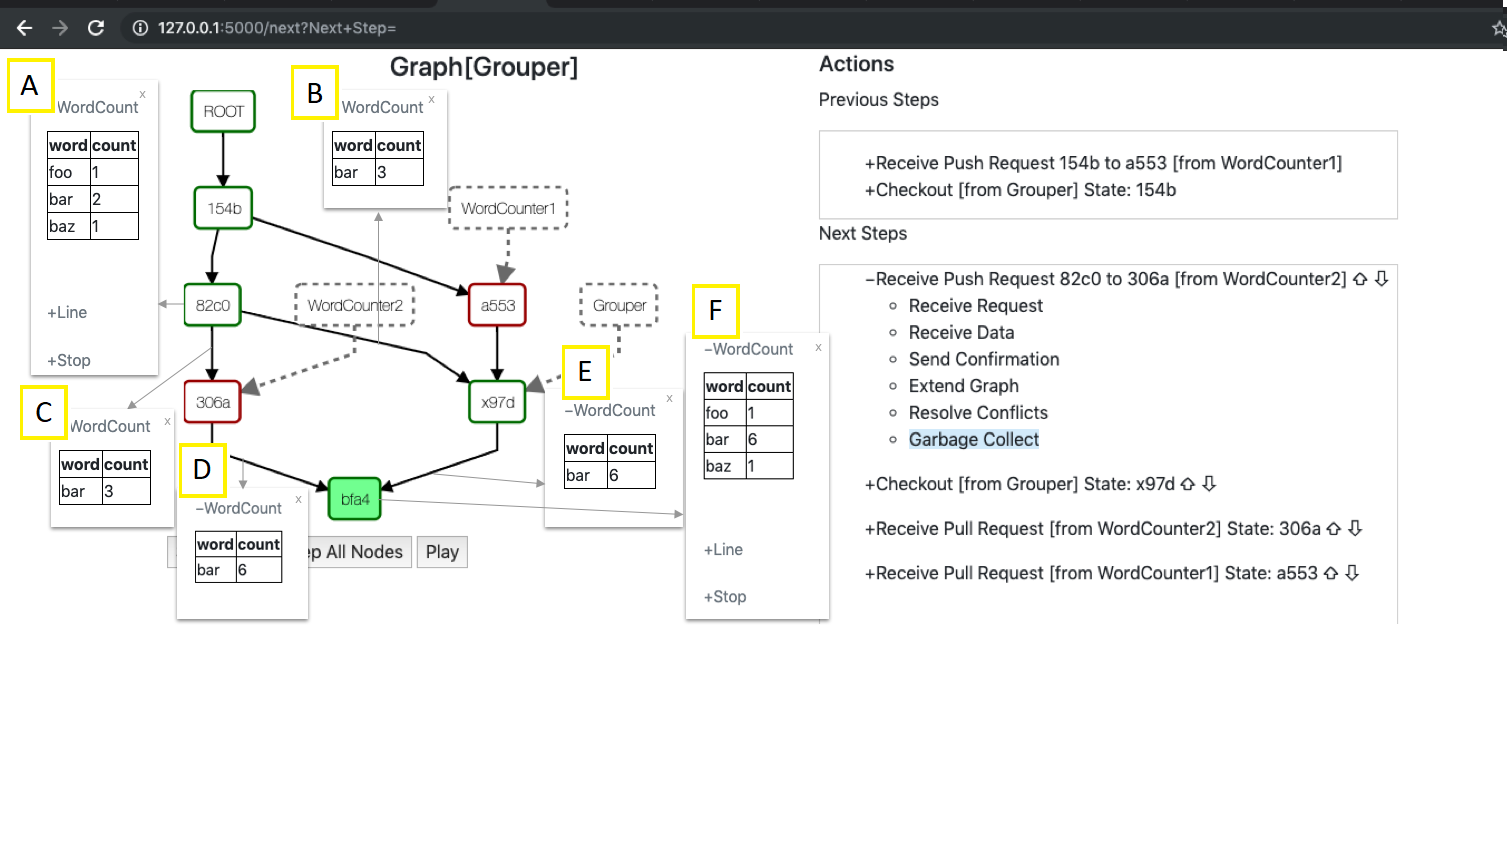
\includegraphics[width=\textwidth]{images/grouper_after_push_resp.png}
%\includegraphics[width=\textwidth]{images/Graph_with_action_state_v4.png}
\caption{Debugger view at Grouper showing response to a {\em push}  request.}
\label{fig:after_push_resp}
\end{figure*}

% What is the state of the version history at breakpoint
The version history contains seven versions. Starting from the top, we have ROOT again as the start version. Version 154b happened-after ROOT. All versions that were present between 154b and ROOT, like the version 632e and 3a27, have all been garbage collected. 

% First merge
At 154b, we see a fork in the path. Both versions 82c0 and a553 happened-after 154b, and are siblings. These are concurrent updates and were performed on different GoT nodes. Version 82c0 is bordered green while a553 is bordered in red. This means that update 154b $\rightarrow$ a553 was received by the version history at Grouper after the update 164b $\rightarrow$ 82c0. The GoT node resolved such conflicts using the custom merge function written in Listing~\ref{lst:merge}. The output of the merge function was a new version x97d. Since x97d happened-after both the concurrent versions, 82c0 and a553, the graph was updated with the happened-after relations and x97d has two in-edges. Additionally, each of these edges are associated with a diff that transforms the previous version to the version at x97d.

% Second merge
Over the course of execution, another concurrent update was performed with the update 82c0 $\rightarrow$ 306a being concurrent with previously resolved conflict. Another conflict resolution is performed using the merge function. A new resolved version bfa4 is created having a happened-after relation with both 306a, and x97d. The version history is updated to show these relations and the version bfa4 is marked as the current HEAD version of the version history at Grouper.

% GC reference
Looking at the dotted line relations, we see that the snapshot at Grouper is at the version x97d. Additionally, the last know versions of WordCounter1 and WordCounter2 are a553, and 306a, respectively.

% Finding the bug
The state at version bfa4 is shown in the tooltip F. The tooltip shows us three WordCount objects and the WordCount object for the word `bar' has a count of six, showing us why the conditional breakpoint was hit. Looking at the version at the start of the merge, 82c0, in the tooltip A, we see that the count of `bar' is two. The diffs associated with 82c0 $\rightarrow$ 306a (tooltip C) and 82c0 $\rightarrow$ x97d (tooltip B) both update the count of `bar' to three. This means that both WordCounter1 and WordCounter2 had the count of `bar' as two, and observed a `bar' token updating the count concurrently to three. At the end of the merge function, this count is set to six, and can be see in the diffs for both 306a $\rightarrow$ bfa4 (tooltip D) and x97d $\rightarrow$ bfa4 (tooltip E). This means that the error is in the merge function. We can see that the merge function in Listing~\ref{lst:merge}, on detecting a conflicting count, simply adds up the counts. So receiving two counts of three, would result in a count of six. However, the actual increment in each update is actually just one. The right way to merge counts would be to find the total change in count and add it to the original count. We can fix the code as shown in Listing~\ref{lst:correct_merge} and the word counting application gives the right output.

\begin{lstlisting}[language=Python,basicstyle=\small, numbers=left,
label=lst:correct_merge, captionpos=b, caption=Merge function used at the Grouper node.]
def merge(conf_iter,orig_df,
          your_df,their_df):
    your_df.update_not_conflicting(
        their_df)
    for orig,yours,theirs in conf_iter:
        assert isinstance(
            yours,WordCounter)
        yours.count += theirs.count
        if orig: # False if new objects.
            yours.count -= orig.count
    return your_df
\end{lstlisting}

This bug was found quite easily because GoTcha exposes the version history. By looking at the evolution of the version history, even though the error had already occurred, we could see in which type of state change the error occurred in. In this case, we could see that the version state was correct before the merge function, but after the reconciliation of two correct states, the state was wrong, telling us that the error was in the custom merge function. GoTcha exposes bugs in a Spacetime application in the same way a tool viewing git history can help find the commit that caused a bug in the code. Instead of the evolution of the files being looked at, GoTcha looks at the evolution of the state at each node.